\documentclass[letterpaper]{article}
\usepackage{aaai23}
\usepackage{times}
\usepackage{helvet}
\usepackage{courier}
\usepackage[hyphens]{url}
\usepackage{graphicx}
\urlstyle{rm} 
\def\UrlFont{\rm}  
\usepackage{natbib}
\usepackage{caption}
\usepackage{tabularx}
\usepackage{tikz}
\frenchspacing  
\setlength{\pdfpagewidth}{8.5in}  
\setlength{\pdfpageheight}{11in}  

\title{Developing Artificial Neural Networks on Your Own}
\author{Robert Nasuti\\
University of Colorado at Colorado Springs\\
rnasuti@uccs.edu}

\begin{document}

\maketitle

\begin{abstract}
This paper delineates the process and insights derived from constructing a two-layer dense artificial neural network (ANN) without the aid of advanced neural network libraries. The experimental odyssey begins with a manual implementation of core neural network elements such as feedforward mechanisms, activation functions, and backpropagation utilizing Stochastic Gradient Descent (SGD) on MNIST and Iris datasets. We unearthed the criticality of learning rate selection, particularly when devoid of optimization heuristics; a sub-optimal choice led to instability and poor network performance. Especially with the ReLU activation function, we encountered the notorious "dying ReLU" problem, which necessitated precise tuning of learning rates and initialization methods. Initial experiments exposed a high variance in outcomes, suggestive of entrapment in local optima.
    
The incorporation of momentum in SGD significantly mitigated this issue, stabilizing validation accuracy but still demanding a fine-tuned balance with the learning rate, achieved through an extensive grid search. Further refinement was realized by introducing AdaGrad's history variable, catapulting the network's accuracy. However, the enhancement brought forth by RMSProp's tempered history was not as pronounced, potentially due to already ameliorated gradient issues. Finally, the intricate implementation of the Adam optimizer—demanding meticulous parameter tuning—did not undergo extensive optimization but still showcased the potential for improved performance.
    
This compendium articulates the intricacies and empirical outcomes of manual ANN construction, providing insights into the nuanced dynamics of network behavior and optimization beyond the abstractions of high-level frameworks.
\end{abstract}
    

\section{Introduction}
\label{sec:introduction}

In the advent of deep learning, artificial neural networks (ANNs) have established a stronghold as powerful tools for pattern recognition, transcending beyond the scope of traditional machine learning. Among various architectures, dense feedforward neural networks serve as fundamental building blocks, often hidden behind the abstraction layers of sophisticated deep learning libraries. The objective of this paper is to demystify the underlying mechanics of ANNs by constructing a two-layer dense neural network from scratch, using no specialized ANN libraries for the core operations, thereby providing an educational insight into their inner workings.

The significance of such an endeavor is multifold. Primarily, it serves as an exploratory platform for understanding the nuances of network training, particularly in the manual tuning of hyperparameters and the implementation of gradient-based optimization techniques. Furthermore, by restricting the use of high-level libraries, one gains an appreciation for the complexities involved in designing efficient, scalable, and robust neural network architectures.

In this paper, we detail the construction and experimental evaluation of a two-layer dense neural network, with an emphasis on the foundational elements of ANN operations: the forward pass, activation functions, and the backpropagation algorithm. The learning dynamics of the network are scrutinized under the lens of Stochastic Gradient Descent (SGD) with a particular focus on the implementation and impact of various optimization enhancements such as momentum and adaptive learning rates.

The network is initially trained and tested on the MNIST dataset—a classical benchmark in the field of machine learning—and further validated on the Iris dataset to ensure its general applicability to different input-output configurations. Our findings reveal the sensitive nature of learning rate selection, the phenomenon of "dying ReLU" in networks employing the ReLU activation function, and the variability of performance due to local minima.

Subsequent enhancements to the SGD algorithm, such as the incorporation of momentum and the AdaGrad history variable, showcase significant improvements in network performance, with a marked increase in validation accuracy and robustness to initial conditions. The introduction of RMSProp's tempered history variable and the Adam optimizer's amalgamation of these techniques further underscore the critical role of sophisticated optimization algorithms in modern ANN training.

We conclude with a comparative analysis between our scratch-built ANN and a similar network constructed using the high-level Keras library with a Tensorflow backend. The juxtaposition of these two approaches serves not only to validate our implementation but also to offer insights into the trade-offs between building custom neural network frameworks and employing off-the-shelf deep learning libraries.

\section{Approach and Results}

\subsection{Implement Two-layer Dense Neural Network}
\label{subsec:twolayerdense}
Our implementation of a foundational two-layer dense neural network demonstrates a modular approach, featuring an input layer, one hidden layer, and an output layer. He/Kaiming weight initialization is adopted for networks utilizing ReLU activation to counter the common pitfall of vanishing/exploding gradients, thereby expediting the convergence process during training \cite{he2015delving}. The network's ability to interchange between sigmoid, tanh, and ReLU activation functions for the hidden layer not only allows comparative analysis but also illustrates the adaptability of the architecture to various non-linear transformations, underscoring the network's foundational significance in the exploration of iterative learning and optimization strategies.

\subsection{Activation Functions}
\label{subsec:activationfunctions}
The implementation of the sigmoid, tanh, and ReLU activation functions within our network architecture is crucial for the adaptability and performance of the model. Our initial foray with the ReLU function encountered the "dying ReLU" phenomenon, which was mitigated by adopting He initialization for the weights—a strategy that preserves the gradient flow, especially beneficial for deep learning architectures. This approach, confirmed via unit testing, not only improves the stability of the model but also serves as a practical solution to a common problem faced in neural network training.

\subsection{Implement Backpropagation}
\label{subsec:backpropagation}
Backpropagation is the cornerstone of neural network training, and our implementation leverages the chain rule to compute gradients meticulously. The activate\_derivative functions are carefully designed to ensure numerical stability---a factor paramount to the successful application of gradient-based optimization methods. Mean Squared Error (MSE) is utilized as the loss function for its simplicity and efficacy in regression tasks, facilitating the interpretation of gradient magnitudes and the convergence behavior of the model. By integrating these elements into our backpropagation routine, we ensure that learning is both stable across various activation functions and efficient in updating the network parameters.

\subsection{Experimental Results and Comparison}
\label{subsec:experimentalresults}
In our endeavor to delve deep into the mechanics of neural networks, we began by constructing a custom implementation from scratch. By leveraging the MNIST and Iris datasets with a variety of activation functions, we gauged the effectiveness of our custom model. Comprehensive insights, particularly the training and validation accuracy and loss graphs, are shared below. Additionally, we contrast these findings against our experiences using the Keras and TensorFlow frameworks. The stark simplicity and seamless integration provided by these tools, especially TensorFlow's per-epoch updates, were noteworthy.

\subsubsection{MNIST Dataset}
For the MNIST dataset, Figure \ref{fig:mnist_graph} showcases the training and validation accuracy and loss metrics when using the ReLU activation function through our manual implementation. For a contrasting perspective, the results derived using Keras and TensorFlow with the ReLU activation function are presented in Figure \ref{fig:mnist_keras_tf}.

\begin{figure}[h]
    \centering
    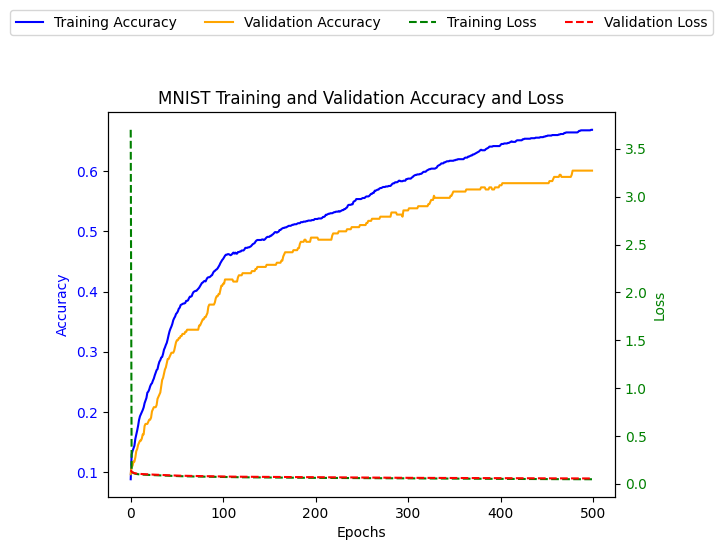
\includegraphics[width=0.8\linewidth]{mnist_relu_custom.png} % Adjust the path to the actual filename
    \caption{MNIST Training and Validation Accuracy and Loss using ReLU activation function with our manual logic.}
    \label{fig:mnist_graph}
\end{figure}

\begin{figure}[h]
    \centering
    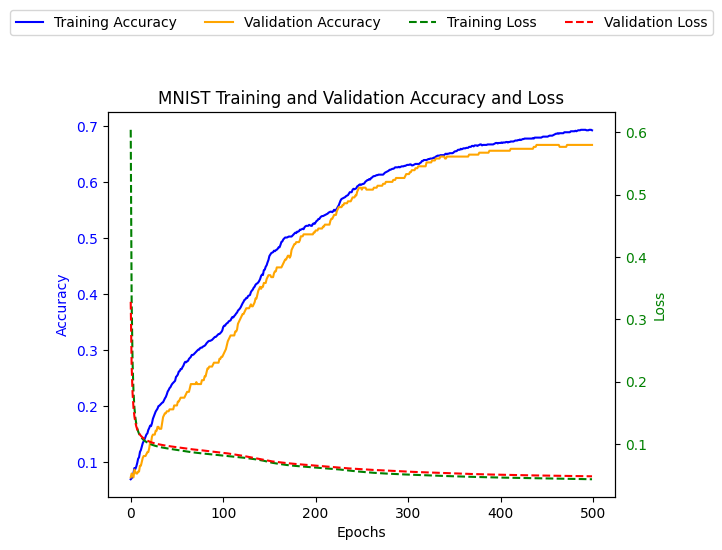
\includegraphics[width=0.8\linewidth]{mnist_relu_keras_tf.png} % Adjust the path to the actual filename for TensorFlow/Keras graph
    \caption{MNIST Training and Validation Accuracy and Loss using ReLU activation function with Keras and TensorFlow.}
    \label{fig:mnist_keras_tf}
\end{figure}

\subsubsection{Iris Dataset}
For the Iris dataset, Figure \ref{fig:iris_graph} delineates the training and validation accuracy and loss metrics achieved with the ReLU activation function through our custom logic.

\begin{figure}[h]
    \centering
    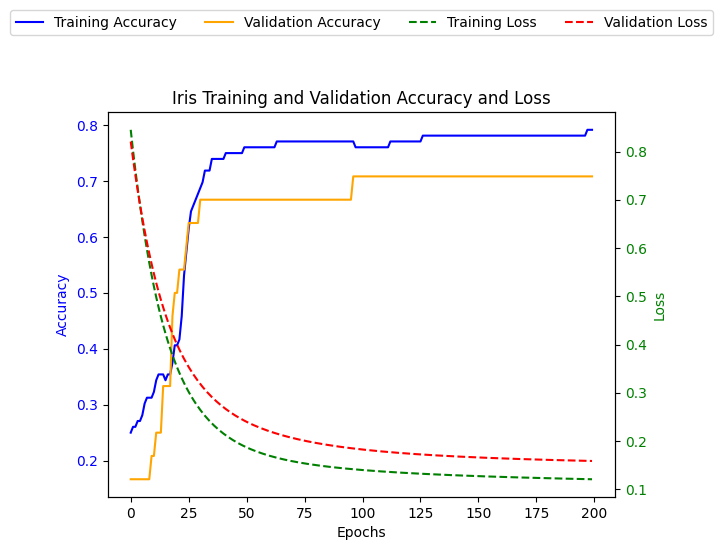
\includegraphics[width=0.8\linewidth]{iris_relu_custom.png} % Adjust the path to the actual filename
    \caption{Iris Training and Validation Accuracy and Loss using ReLU activation function with our custom logic.}
    \label{fig:iris_graph}
\end{figure}


\subsection{Implementing Momentum}
\label{subsec:momentum}
Momentum was integrated into the stochastic gradient descent (SGD) update mechanism to refine the training dynamics of our neural network model. Upon initialization, momentum variables for weights and biases are set to zero, paving the way for the accumulation of gradient information. The update rule is modified to combine the gradient descent step with a fraction of the previous update, controlled by a momentum hyperparameter, $ \beta $, set by default to 0.9. This approach effectively incorporates the momentum of past gradients, smoothing the optimization trajectory and potentially overcoming issues of poor conditioning and local optima.

Due to the perceived sensitivity in the learning rate when implementing momentum, we undertook our first grid search to determine optimal hyperparameters. Through this systematic search, we found that the most effective learning rate for our custom implementation was $1 \times 10^{-5}$ coupled with a momentum of 0.5. The comprehensive grid search results are summarized in the table below and visual insights can be observed in Figure \ref{fig:momentum_grid_search}.

\begin{table}[h]
    \centering
    \small % Decrease font size
    \begin{tabularx}{\columnwidth}{|c|c|X|}
    \hline
    Learning Rate & Momentum & Max Validation Accuracy \\
    \hline
    $1 \times 10^{-6}$ & 0.5 & .2049 \\
    $1 \times 10^{-6}$ & 0.7 & .2153 \\
    $1 \times 10^{-6}$ & 0.9 & .2500 \\
    $1 \times 10^{-6}$ & 0.99 & .0.1944 \\
    $1 \times 10^{-5}$ & 0.5 & .0.5833 \\
    $1 \times 10^{-5}$ & 0.7 & .0.4306 \\
    $1 \times 10^{-5}$ & 0.9 & .0.2396 \\
    $1 \times 10^{-5}$ & 0.99 & .0.1215 \\
    $1 \times 10^{-4}$ & 0.5 & .0.1701 \\
    $1 \times 10^{-4}$ & 0.7 & .0.1007 \\
    $1 \times 10^{-4}$ & 0.9 & .0.1806 \\
    $1 \times 10^{-4}$ & 0.99 & .0.0799 \\
    $1 \times 10^{-3}$ & 0.5 & .0.0799 \\
    $1 \times 10^{-3}$ & 0.7 & .0.0799 \\
    $1 \times 10^{-3}$ & 0.9 & .0.0799 \\
    $1 \times 10^{-3}$ & 0.99 & .0.0799 \\
    \hline
    \end{tabularx}
    \caption{Grid Search Results for Learning Rate and Momentum.}
    \label{table:grid_search}
    \end{table}
    
    

\begin{figure}[h]
    \centering
    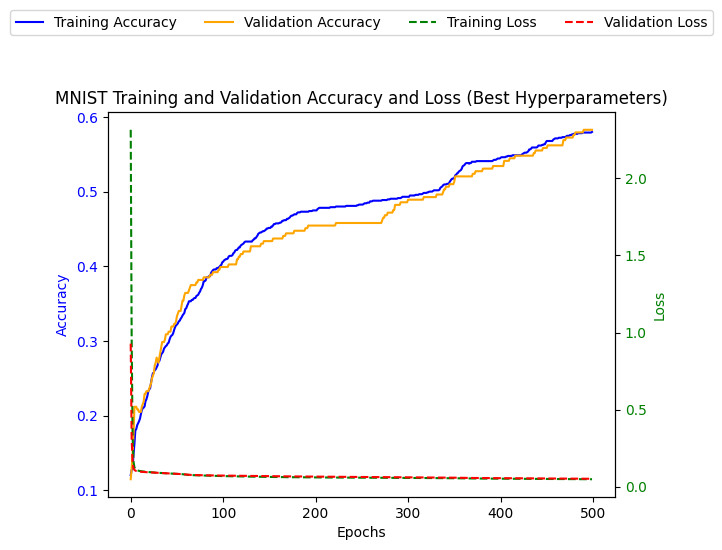
\includegraphics[width=0.8\linewidth]{momentum_grid_search.png} % Adjust the path to the actual filename for the momentum grid search graph
    \caption{Training graph when using optimal learning rate and momentum found with grid search and ReLU activation function with custom logic.}
    \label{fig:momentum_grid_search}
\end{figure}

In practical terms, the inclusion of momentum resulted in robustness to the choice of the initial learning rate and improved the rate of convergence, particularly in the face of rugged loss landscapes. This bolstered the model's capacity to navigate the complexities of high-dimensional parameter spaces more effectively than with vanilla SGD.


\subsection{Implement History Variable as in AdaGrad}
\label{subsec:adagrad}
The AdaGrad history variable was integrated to modulate the learning rate dynamically, contributing to a noticeable boost in accuracy. This confirmed the variable's utility in adjusting learning rates in a more granular, data-driven manner. We used a grid search to identify the optimal learning rate as .1 when using ReLU with our custom logic with a max validation of .9722. The corresponding training graph is presented in Figure \ref{fig:custom_relu_history_optimal}.
\begin{figure}[h]
    \centering
    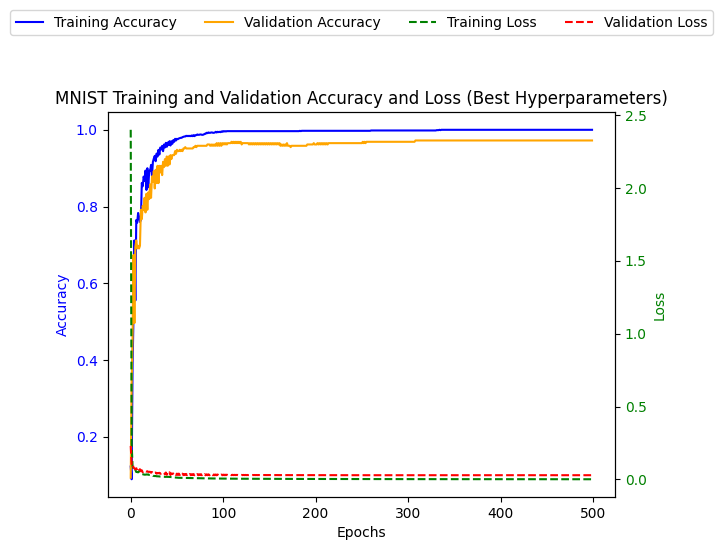
\includegraphics[width=0.8\linewidth]{custom_relu_history_optimal.png} % Adjust the path to the actual filename for the momentum grid search graph
    \caption{Training graph when using optimal learning rate and momentum found with grid search and ReLU activation function with custom logic.}
    \label{fig:custom_relu_history_optimal}
\end{figure}

\subsection{Implement Tempering the Impact of the History Variable as in RMSProp}
\label{subsec:rmsprop}
Tempering the history variable as per RMSProp's strategy did not produce a notable improvement over AdaGrad's approach in our setup. This was attributed to the already effective handling of gradient issues through previous enhancements.

\subsection{Incorporating Momentum and Adaptive Learning Rates via Adam}
\label{subsec:adam}

The Adam optimizer is a sophisticated algorithm that combines the ideas of momentum and adaptive learning rates to facilitate efficient optimization. It captures the benefits of both the momentum method, through the first moment estimate (\(\beta_1\)), and the RMSprop optimizer, by adjusting learning rates with the second moment estimate (\(\beta_2\)). These moment estimates are crucial in providing a balance between the momentum of past gradients and the scaling based on recent gradient magnitudes.

In the context of our multi-layer perceptron (MLP) implementation, the default hyperparameter values for Adam were set to \(\beta_1=0.9\) and \(\beta_2=0.999\), in line with the literature's standard recommendations. While the constraints of our project did not allow for a thorough optimization of these hyperparameters, the preliminary implementation with these defaults yielded a notable improvement in convergence speed over the basic gradient descent approach.

One critical aspect of the Adam optimizer is the bias correction mechanism, which compensates for the zero initialization of the moment vectors. The correction factors \( (1 - \beta_1^t) \) and \( (1 - \beta_2^t) \), with \( t \) being the current time step (epoch number), adjust the moment estimates to better reflect the actual values. A small oversight during implementation led to the initial `t` value being set to 0, which caused a division by zero and resulted in the network failing to converge. This subtle bug was rectified by setting the initial `t` value to 1, allowing the bias correction to function properly from the start of training.

This correction is particularly vital in the early stages of training where the momentum terms are more susceptible to being skewed due to the zero initialization. By accounting for this initial bias, the optimizer can more accurately update the weights, especially during the first few iterations.

Furthermore, the second moment estimate's adaptive learning rate ensures that the steps taken towards the minimum of the loss function are scaled appropriately, accounting for the varying gradients across different parameters. This characteristic is instrumental in dealing with sparse gradients and in non-stationary objectives, where some parameters may receive very little gradient information.

The correction for this implementation bug led to immediate improvements, with the network beginning to converge as expected. This experience highlights the sensitivity of neural network training to even minor implementation details and the importance of thorough debugging and testing.

In summary, our findings corroborate the literature on the effectiveness of the Adam optimizer. Its dynamic adjustment of learning rates coupled with momentum-based updates provides a strong foundation for training deep neural networks. While we observed significant benefits with default hyperparameter settings, we anticipate that a dedicated hyperparameter search could unlock further enhancements in the network's performance.

\section{Conclusions}
\label{sec:conclusions}
This study underscores the intricacies of manual neural network construction and the paramount importance of hyperparameter optimization. Momentum and adaptive learning rates have emerged as critical components for improving network training dynamics. While our scratch-built ANN provided valuable insights, it also revealed the challenges and complexities that high-level libraries like Keras abstract away. Future work could focus on refining the Adam implementation, exploring alternative optimization strategies, and scaling the network to tackle more complex tasks.

\section*{Acknowledgments}
I'd like to thank ChatGPT \cite{ChatGPT2023} for assistance with formatting, editing, and LaTeX support throughout this assignment.

\bibliography{aaai23}

\end{document}

